%% bare_conf.tex
%% V1.3
%% 2007/01/11
%% by Michael Shell
%% See:
%% http://www.michaelshell.org/
%% for current contact information.
%%
%% This is a skeleton file demonstrating the use of IEEEtran.cls
%% (requires IEEEtran.cls version 1.7 or later) with an IEEE conference paper.
%%
%% Support sites:
%% http://www.michaelshell.org/tex/ieeetran/
%% http://www.ctan.org/tex-archive/macros/latex/contrib/IEEEtran/
%% and
%% http://www.ieee.org/

%%*************************************************************************
%% Legal Notice:
%% This code is offered as-is without any warranty either expressed or
%% implied; without even the implied warranty of MERCHANTABILITY or
%% FITNESS FOR A PARTICULAR PURPOSE! 
%% User assumes all risk.
%% In no event shall IEEE or any contributor to this code be liable for
%% any damages or losses, including, but not limited to, incidental,
%% consequential, or any other damages, resulting from the use or misuse
%% of any information contained here.
%%
%% All comments are the opinions of their respective authors and are not
%% necessarily endorsed by the IEEE.
%%
%% This work is distributed under the LaTeX Project Public License (LPPL)
%% ( http://www.latex-project.org/ ) version 1.3, and may be freely used,
%% distributed and modified. A copy of the LPPL, version 1.3, is included
%% in the base LaTeX documentation of all distributions of LaTeX released
%% 2003/12/01 or later.
%% Retain all contribution notices and credits.
%% ** Modified files should be clearly indicated as such, including  **
%% ** renaming them and changing author support contact information. **
%%
%% File list of work: IEEEtran.cls, IEEEtran_HOWTO.pdf, bare_adv.tex,
%%                    bare_conf.tex, bare_jrnl.tex, bare_jrnl_compsoc.tex
%%*************************************************************************

% *** Authors should verify (and, if needed, correct) their LaTeX system  ***
% *** with the testflow diagnostic prior to trusting their LaTeX platform ***
% *** with production work. IEEE's font choices can trigger bugs that do  ***
% *** not appear when using other class files.                            ***
% The testflow support page is at:
% http://www.michaelshell.org/tex/testflow/



% Note that the a4paper option is mainly intended so that authors in
% countries using A4 can easily print to A4 and see how their papers will
% look in print - the typesetting of the document will not typically be
% affected with changes in paper size (but the bottom and side margins will).
% Use the testflow package mentioned above to verify correct handling of
% both paper sizes by the user's LaTeX system.
%
% Also note that the "draftcls" or "draftclsnofoot", not "draft", option
% should be used if it is desired that the figures are to be displayed in
% draft mode.
%
\documentclass[10pt,conference,compsocconf]{IEEEtran}
%\documentclass[10pt]{IEEEtran}
\usepackage{times}

\usepackage{caption}
\captionsetup{font=footnotesize,justification=centering,labelsep=period}

% Add the compsoc option for Computer Society conferences.
%
% If IEEEtran.cls has not been installed into the LaTeX system files,
% manually specify the path to it like:
% \documentclass[conference]{../sty/IEEEtran}





% Some very useful LaTeX packages include:
% (uncomment the ones you want to load)


% *** MISC UTILITY PACKAGES ***
%
%\usepackage{ifpdf}
% Heiko Oberdiek's ifpdf.sty is very useful if you need conditional
% compilation based on whether the output is pdf or dvi.
% usage:
% \ifpdf
%   % pdf code
% \else
%   % dvi code
% \fi
% The latest version of ifpdf.sty can be obtained from:
% http://www.ctan.org/tex-archive/macros/latex/contrib/oberdiek/
% Also, note that IEEEtran.cls V1.7 and later provides a builtin
% \ifCLASSINFOpdf conditional that works the same way.
% When switching from latex to pdflatex and vice-versa, the compiler may
% have to be run twice to clear warning/error messages.






% *** CITATION PACKAGES ***
%
%\usepackage{cite}
% cite.sty was written by Donald Arseneau
% V1.6 and later of IEEEtran pre-defines the format of the cite.sty package
% \cite{} output to follow that of IEEE. Loading the cite package will
% result in citation numbers being automatically sorted and properly
% "compressed/ranged". e.g., [1], [9], [2], [7], [5], [6] without using
% cite.sty will become [1], [2], [5]--[7], [9] using cite.sty. cite.sty's
% \cite will automatically add leading space, if needed. Use cite.sty's
% noadjust option (cite.sty V3.8 and later) if you want to turn this off.
% cite.sty is already installed on most LaTeX systems. Be sure and use
% version 4.0 (2003-05-27) and later if using hyperref.sty. cite.sty does
% not currently provide for hyperlinked citations.
% The latest version can be obtained at:
% http://www.ctan.org/tex-archive/macros/latex/contrib/cite/
% The documentation is contained in the cite.sty file itself.






% *** GRAPHICS RELATED PACKAGES ***
%
\ifCLASSINFOpdf
  \usepackage[pdftex]{graphicx}
%  declare the path(s) where your graphic files are
  \graphicspath{{figures}}
%  and their extensions so you won't have to specify these with
%  every instance of \includegraphics
  \DeclareGraphicsExtensions{.pdf,.jpeg,.png}
\else
  % or other class option (dvipsone, dvipdf, if not using dvips). graphicx
  % will default to the driver specified in the system graphics.cfg if no
  % driver is specified.
  % \usepackage[dvips]{graphicx}
  % declare the path(s) where your graphic files are
  % \graphicspath{{../eps/}}
  % and their extensions so you won't have to specify these with
  % every instance of \includegraphics
  % \DeclareGraphicsExtensions{.eps}
\fi
% graphicx was written by David Carlisle and Sebastian Rahtz. It is
% required if you want graphics, photos, etc. graphicx.sty is already
% installed on most LaTeX systems. The latest version and documentation can
% be obtained at: 
% http://www.ctan.org/tex-archive/macros/latex/required/graphics/
% Another good source of documentation is "Using Imported Graphics in
% LaTeX2e" by Keith Reckdahl which can be found as epslatex.ps or
% epslatex.pdf at: http://www.ctan.org/tex-archive/info/
%
% latex, and pdflatex in dvi mode, support graphics in encapsulated
% postscript (.eps) format. pdflatex in pdf mode supports graphics
% in .pdf, .jpeg, .png and .mps (metapost) formats. Users should ensure
% that all non-photo figures use a vector format (.eps, .pdf, .mps) and
% not a bitmapped formats (.jpeg, .png). IEEE frowns on bitmapped formats
% which can result in "jaggedy"/blurry rendering of lines and letters as
% well as large increases in file sizes.
%
% You can find documentation about the pdfTeX application at:
% http://www.tug.org/applications/pdftex





% *** MATH PACKAGES ***
%
%\usepackage[cmex10]{amsmath}
% A popular package from the American Mathematical Society that provides
% many useful and powerful commands for dealing with mathematics. If using
% it, be sure to load this package with the cmex10 option to ensure that
% only type 1 fonts will utilized at all point sizes. Without this option,
% it is possible that some math symbols, particularly those within
% footnotes, will be rendered in bitmap form which will result in a
% document that can not be IEEE Xplore compliant!
%
% Also, note that the amsmath package sets \interdisplaylinepenalty to 10000
% thus preventing page breaks from occurring within multiline equations. Use:
%\interdisplaylinepenalty=2500
% after loading amsmath to restore such page breaks as IEEEtran.cls normally
% does. amsmath.sty is already installed on most LaTeX systems. The latest
% version and documentation can be obtained at:
% http://www.ctan.org/tex-archive/macros/latex/required/amslatex/math/





% *** SPECIALIZED LIST PACKAGES ***
%
%\usepackage{algorithmic}
% algorithmic.sty was written by Peter Williams and Rogerio Brito.
% This package provides an algorithmic environment fo describing algorithms.
% You can use the algorithmic environment in-text or within a figure
% environment to provide for a floating algorithm. Do NOT use the algorithm
% floating environment provided by algorithm.sty (by the same authors) or
% algorithm2e.sty (by Christophe Fiorio) as IEEE does not use dedicated
% algorithm float types and packages that provide these will not provide
% correct IEEE style captions. The latest version and documentation of
% algorithmic.sty can be obtained at:
% http://www.ctan.org/tex-archive/macros/latex/contrib/algorithms/
% There is also a support site at:
% http://algorithms.berlios.de/index.html
% Also of interest may be the (relatively newer and more customizable)
% algorithmicx.sty package by Szasz Janos:
% http://www.ctan.org/tex-archive/macros/latex/contrib/algorithmicx/




% *** ALIGNMENT PACKAGES ***
%
%\usepackage{array}
% Frank Mittelbach's and David Carlisle's array.sty patches and improves
% the standard LaTeX2e array and tabular environments to provide better
% appearance and additional user controls. As the default LaTeX2e table
% generation code is lacking to the point of almost being broken with
% respect to the quality of the end results, all users are strongly
% advised to use an enhanced (at the very least that provided by array.sty)
% set of table tools. array.sty is already installed on most systems. The
% latest version and documentation can be obtained at:
% http://www.ctan.org/tex-archive/macros/latex/required/tools/


%\usepackage{mdwmath}
%\usepackage{mdwtab}
% Also highly recommended is Mark Wooding's extremely powerful MDW tools,
% especially mdwmath.sty and mdwtab.sty which are used to format equations
% and tables, respectively. The MDWtools set is already installed on most
% LaTeX systems. The lastest version and documentation is available at:
% http://www.ctan.org/tex-archive/macros/latex/contrib/mdwtools/


% IEEEtran contains the IEEEeqnarray family of commands that can be used to
% generate multiline equations as well as matrices, tables, etc., of high
% quality.


%\usepackage{eqparbox}
% Also of notable interest is Scott Pakin's eqparbox package for creating
% (automatically sized) equal width boxes - aka "natural width parboxes".
% Available at:
% http://www.ctan.org/tex-archive/macros/latex/contrib/eqparbox/





% *** SUBFIGURE PACKAGES ***
%\usepackage[tight,footnotesize]{subfigure}
% subfigure.sty was written by Steven Douglas Cochran. This package makes it
% easy to put subfigures in your figures. e.g., "Figure 1a and 1b". For IEEE
% work, it is a good idea to load it with the tight package option to reduce
% the amount of white space around the subfigures. subfigure.sty is already
% installed on most LaTeX systems. The latest version and documentation can
% be obtained at:
% http://www.ctan.org/tex-archive/obsolete/macros/latex/contrib/subfigure/
% subfigure.sty has been superceeded by subfig.sty.



%\usepackage[caption=false]{caption}
%\usepackage[font=footnotesize]{subfig}
% subfig.sty, also written by Steven Douglas Cochran, is the modern
% replacement for subfigure.sty. However, subfig.sty requires and
% automatically loads Axel Sommerfeldt's caption.sty which will override
% IEEEtran.cls handling of captions and this will result in nonIEEE style
% figure/table captions. To prevent this problem, be sure and preload
% caption.sty with its "caption=false" package option. This is will preserve
% IEEEtran.cls handing of captions. Version 1.3 (2005/06/28) and later 
% (recommended due to many improvements over 1.2) of subfig.sty supports
% the caption=false option directly:
%\usepackage[caption=false,font=footnotesize]{subfig}
%
% The latest version and documentation can be obtained at:
% http://www.ctan.org/tex-archive/macros/latex/contrib/subfig/
% The latest version and documentation of caption.sty can be obtained at:
% http://www.ctan.org/tex-archive/macros/latex/contrib/caption/




% *** FLOAT PACKAGES ***
%
%\usepackage{fixltx2e}
% fixltx2e, the successor to the earlier fix2col.sty, was written by
% Frank Mittelbach and David Carlisle. This package corrects a few problems
% in the LaTeX2e kernel, the most notable of which is that in current
% LaTeX2e releases, the ordering of single and double column floats is not
% guaranteed to be preserved. Thus, an unpatched LaTeX2e can allow a
% single column figure to be placed prior to an earlier double column
% figure. The latest version and documentation can be found at:
% http://www.ctan.org/tex-archive/macros/latex/base/



%\usepackage{stfloats}
% stfloats.sty was written by Sigitas Tolusis. This package gives LaTeX2e
% the ability to do double column floats at the bottom of the page as well
% as the top. (e.g., "\begin{figure*}[!b]" is not normally possible in
% LaTeX2e). It also provides a command:
%\fnbelowfloat
% to enable the placement of footnotes below bottom floats (the standard
% LaTeX2e kernel puts them above bottom floats). This is an invasive package
% which rewrites many portions of the LaTeX2e float routines. It may not work
% with other packages that modify the LaTeX2e float routines. The latest
% version and documentation can be obtained at:
% http://www.ctan.org/tex-archive/macros/latex/contrib/sttools/
% Documentation is contained in the stfloats.sty comments as well as in the
% presfull.pdf file. Do not use the stfloats baselinefloat ability as IEEE
% does not allow \baselineskip to stretch. Authors submitting work to the
% IEEE should note that IEEE rarely uses double column equations and
% that authors should try to avoid such use. Do not be tempted to use the
% cuted.sty or midfloat.sty packages (also by Sigitas Tolusis) as IEEE does
% not format its papers in such ways.





% *** PDF, URL AND HYPERLINK PACKAGES ***
%
%\usepackage{url}
% url.sty was written by Donald Arseneau. It provides better support for
% handling and breaking URLs. url.sty is already installed on most LaTeX
% systems. The latest version can be obtained at:
% http://www.ctan.org/tex-archive/macros/latex/contrib/misc/
% Read the url.sty source comments for usage information. Basically,
% \url{my_url_here}.





% *** Do not adjust lengths that control margins, column widths, etc. ***
% *** Do not use packages that alter fonts (such as pslatex).         ***
% There should be no need to do such things with IEEEtran.cls V1.6 and later.
% (Unless specifically asked to do so by the journal or conference you plan
% to submit to, of course. )


% correct bad hyphenation here
\hyphenation{op-tical net-works semi-conduc-tor}

%\parskip 6pt plus 2pt minus 1pt
\parskip 3pt plus 2pt minus 1pt

\pagestyle{empty}
\begin{document}
\pagenumbering{gobble}
%
% paper title
% can use linebreaks \\ within to get better formatting as desired
\title{Scalable Long-Stroke Linear Variable Displacement Sensor Using Inexpensive Components and 3D Printing}

%% \title{\textbf{\Large Bare Demo of IEEEtran.cls for
%% Conferences\\[-1.5ex] and subtitle}\\[0.2ex]}

% author names and affiliations
% use a multiple column layout for up to three different
% affiliations
\author{\IEEEauthorblockN{~\\[-0.4ex]\large Keeshan Patel\\[0.3ex]\normalsize}
\IEEEauthorblockA{University of Texas at Austin\\
Email: {\tt keeshanppatel@gmail.com}}
\and
\IEEEauthorblockN{~\\[-0.4ex]\large Robert L. Read\\[0.3ex]\normalsize}
\IEEEauthorblockA{Founder, Public Invention, an educational non-profit.\\
Email: {\tt read.robert@gmail.com}} \\
}

% conference papers do not typically use \thanks and this command
% is locked out in conference mode. If really needed, such as for
% the acknowledgment of grants, issue a \IEEEoverridecommandlockouts
% after \documentclass

% for over three affiliations, or if they all won't fit within the width
% of the page, use this alternative format:
% 
%\author{\IEEEauthorblockN{Michael Shell\IEEEauthorrefmark{1},
%Homer Simpson\IEEEauthorrefmark{2},
%James Kirk\IEEEauthorrefmark{3}, 
%Montgomery Scott\IEEEauthorrefmark{3} and
%Eldon Tyrell\IEEEauthorrefmark{4}}
%\IEEEauthorblockA{\IEEEauthorrefmark{1}School of Electrical and Computer Engineering\\
%Georgia Institute of Technology,
%Atlanta, Georgia 30332--0250\\ Email: see http://www.michaelshell.org/contact.html}
%\IEEEauthorblockA{\IEEEauthorrefmark{2}Twentieth Century Fox, Springfield, USA\\
%Email: homer@thesimpsons.com}
%\IEEEauthorblockA{\IEEEauthorrefmark{3}Starfleet Academy, San Francisco, California 96678-2391\\
%Telephone: (800) 555--1212, Fax: (888) 555--1212}
%\IEEEauthorblockA{\IEEEauthorrefmark{4}Tyrell Inc., 123 Replicant Street, Los Angeles, California 90210--4321}}




% use for special paper notices
%\IEEEspecialpapernotice{(Invited Paper)}




% make the title area
\maketitle


\begin{abstract}
%\boldmath
Displacement sensors measure the change in position of a physical object attached to the sensor. Instruments, such as linear slide potentiometers are inexpensive and robust when such a physical connection is not a problem or even an advantage. However, the currently manufactured slide potentiometers offer only a limited number of size and range choices. Driven by the need to allow arbitrary ranges of displacements and to scale to larger and smaller displacements, we experimented with a simple, inexpensive approach using LEDs and light sensors in a 3D printed chamber. When calibrated in software, the resulting system seems a practical, inexpensive approach to producing displacements sensors of scales larger than and smaller than 10 cm.
\end{abstract}
% IEEEtran.cls defaults to using nonbold math in the Abstract.
% This preserves the distinction between vectors and scalars. However,
% if the conference you are submitting to favors bold math in the abstract,
% then you can use LaTeX's standard command \boldmath at the very start
% of the abstract to achieve this. Many IEEE journals/conferences frown on
% math in the abstract anyway.

% no keywords

\begin{IEEEkeywords}
Anything; Something; Everything else.%
\end{IEEEkeywords}



% For peer review papers, you can put extra information on the cover
% page as needed:
% \ifCLASSOPTIONpeerreview
% \begin{center} \bfseries EDICS Category: 3-BBND \end{center}
% \fi
%
% For peerreview papers, this IEEEtran command inserts a page break and
% creates the second title. It will be ignored for other modes.
\IEEEpeerreviewmaketitle


\section{Introduction}

\subsection{Motivation}

This research grew out of our need to make small sensors of specific sizes which we were unable to easily source.  We are in fact building a net or framework rods which can change their length. This is a “puppet” or “waldo” controller for a larger robot in the same geometry, constructed out of linear actuators. The resulting waldo can be manipulated by hand to cause a corresponding motion in the larger robot. It is like playing with a doll or action figure, to effect a realistic motion.

Ideally, we would be able to construct this “waldo” out of sliding rods that can change their length in any size that we desire. Since we combine the joints using a special joint, the Kwon-Song-Kim joint, that can only be created by 3D printing, it is natural for us to seek a 3D printable solution, even though of course in a perfect world one might order a sensor of any size that could be manufactured with a wide variety of techniques.


\subsection{Mechanism}

In open space, the intensity of light falling on a sensor is inversely proportional to the square of the distance travelled between the source and sensor. When encased in a tube, some fraction of the light is reflected off the walls of the tube, so the light reaching the sensor is does not have a simple mathematical relationship with displacement. However, it is monotone---the light intensity decreases smoothly with increasing displacement, even if the rate of decrease is not easily predictable. Since we always intended to read our sensor value with a microcontroller such as an Arduino, it is simple to perform calibration in software. By using a simple light-and-sensor mechanism in a sliding cylinder with a reflective piston, we construct a displacement sensor with few limits on scaling up or scaling down. By putting the sensor and the light at the same end, we simplify the wiring, although this requires a reflection of the light.


\section{Construction of the Sensor}

We started by gathering the basic materials needed to make the sensor operational. An Arduino Uno microcontroller for its analog to digital converter, an LED as a light source, and a CdS cell for light detection,such as comes with the Arduino Experimenter’s Kit (ARDX) from Adafruit. First, the LED and CdS cell were physically measured and created in AutoDesk Inventor. Then a housing unit was created for the LED and CdS cell with a baffle to separate them so that the LEd did not directly shine on the Cds cell. A piston and cylinder were created to for the housing. Tolerances were checked for the CAD model and then the models were 3D printed. We powered the CdS at 5V and the LED at 3.3V using the Arduino Uno. A resistor was added to the LED circuit to prevent it burning out. The CdS cell was voltage was read by the analog input of the Uno. This procedure was repeated for a smaller version of the sensor as well. In theory the cylinder size can be parametrically controlled to a large number of physical lengths and even diameters.

\begin{figure}
  \centering
  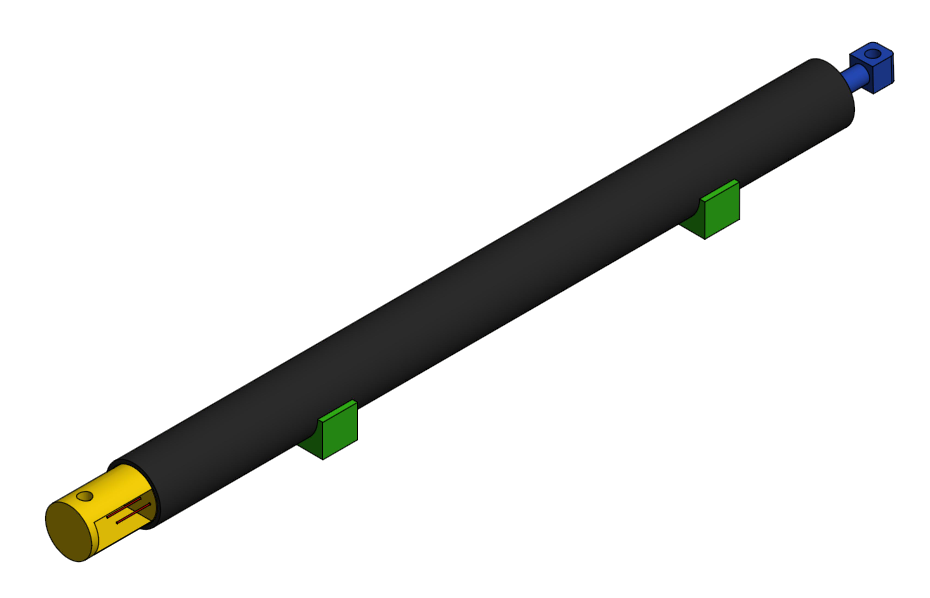
\includegraphics[width=2.5in]{figures/IsometricView.png}
  \caption{Isometric View}  
\end{figure}

\begin{figure}
  \centering
  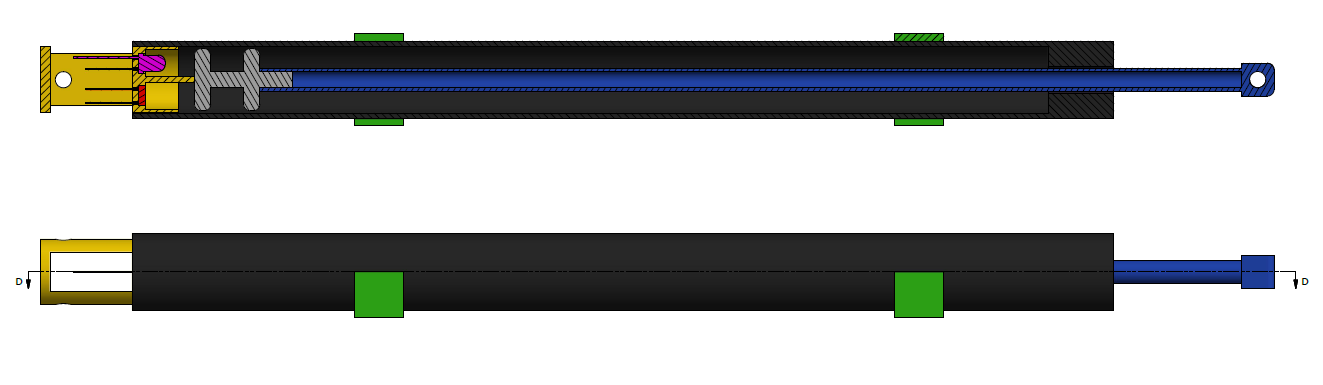
\includegraphics[width=2.5in]{figures/Contracted.png}
  \caption{Contracted View}  
\end{figure}

\begin{figure}
  \centering
  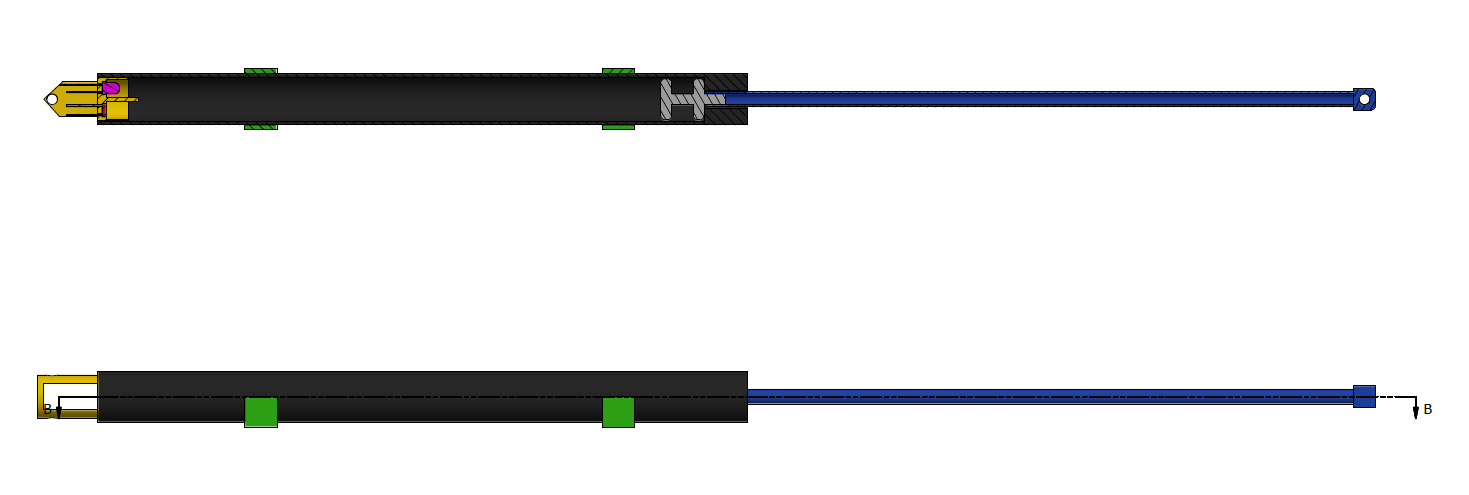
\includegraphics[width=2.5in]{figures/Expanded.png}
  \caption{Expanded View}  
\end{figure}


\section{Electrical Performance}

The charts below show the measured voltage at the CdS cell based on physical change in the displacement of the piston within the cylinder. Initially, we performed a regression analysis, but it soon became clear that digital calibration would be preferred. There was in all cases a smooth monotone relationship between output signal voltage and the position of the piston as seen in the diagrams below. 

Each plot plots the linear displacement as the vertical (Y) axis. In the large sensor this is measured in centimeters. The horizontal line is the digital read of the analog input returned by the Uno, on a scale of 0 to 1023, which is in fact proportional to the voltage via the formula: V = (input * 1000 milivolts)/ 5 = input * 200 millivolts. An digital read of 1000 corresponds to 5V. In the case of the smaller sensor, the scale of displacement is measured in mm.

Observe that using a aluminum foil as the reflector in the large model “linearized” the curve and allowed better separation of values at large displacements of 15 cm or more.

Note that this depends on the bore diameter, the reflectance of the piston head, the kind of LED and CDS cell, as well as the input voltage.

\section{Digital Calibration}

\begin{figure}
  \centering
  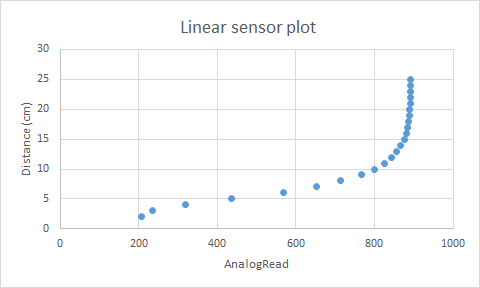
\includegraphics[width=2.5in]{figures/WhiteLargeDistanceVsRead.png}
  \caption{Large Sensor White Tip Distance vs. Voltage}  
\end{figure}

\begin{figure}
  \centering
  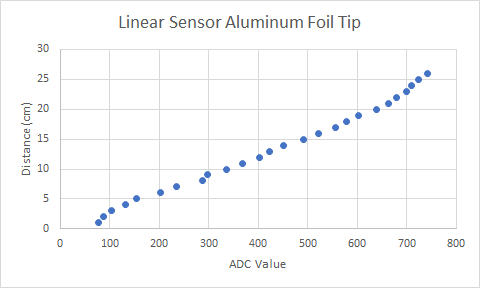
\includegraphics[width=2.5in]{figures/AluminumLargeFoil.png}
  \caption{Large Sensor Aluminum Tip Distance vs. Voltage}  
\end{figure}

\begin{figure}
  \centering
  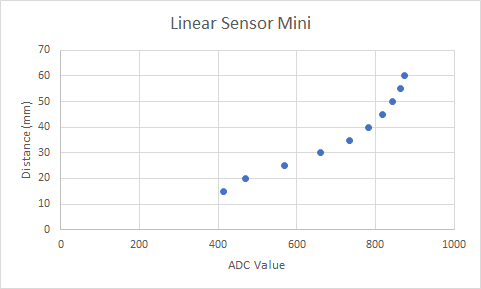
\includegraphics[width=2.5in]{figures/MiniDistanceVsRead.png}
  \caption{Mini Sensor White Tip Distance vs. Voltage}  
\end{figure}


Because the voltage produced by the optical linear sensor is in the common ranges of 0-5V, it is easy to digitize the signal with a standard Analog-to-Digital converter or common hobbyist microcontrollers, such as the Arduino. Although some sensors are carefully designed to allow a directly meaningful voltage level to be output, we assumed that in most cases our sensors would be used by a microcontroller anyway.

The procedure was to wire the LED, photocell, and resistor to the Arduino. A simple Arduino script was used to sample the photocell’s voltage divider once every second. The ADC value from the serial output of the Arduino was recorded for every 1 centimeter from 0 cm to 26 cm.

The results of the experiment were recorded in an excel sheet. Since the Arduino uses a 12 bit ADC, the output of the serial reading range from 0 to 1023. The equation [(measurement)/1023 * 5] was used to map the ADC value to a voltage. 

We have produced Arduino code that performs a simple linear interpolation of data points recorded by hand. The code is available in our GitHub repo: (https://github.com/PubInv/optical-linear-sensor) under the GNU Public License.

\section{Future Work}

This paper explains how to make a calibratable displacement sensor using light intensity as its fundamental mechanism.  

A number of interesting improvements are in theory possible. Perhaps the best, since we are already using 3D printing, is to attempt to create a “digital” displacement 


From this baseline concept of having light as a means of detecting distance, many directions can be taken to improve upon or modify the design for future iterations of the sensor. For instance, in order to decrease the overall footprint of the device, fiber optics could be used to transmit light into a smaller tube rather than having the led taking up space in the tube itself. This would make the circumference of the tube smaller, potentially opening the device to other applications. 

Also, there is potential to make the system digital by changing the geometry of the inside of the tube. Instead of having a hollow tube, chambers and cavities could be made to “catch” the light at a precise distance. This would carry on for multiple intervals and in theory when the light hits one of the cavities there would be a sharp drop in reflectivity and the photocell would be able to detect the change in intensity and distance. 

There are many more directions that could be taken with the optical linear sensor concept and with each modification, a different use for the device could be discovered.


\section{Conclusion}

This paper describes a means of constructing linear position sensors of widely-varying (human-scale) size with 3D printing and cheap electronics components. This invention is released under a Creative Commons license. Because it does not use physical contact as in most pressure sensors or linear potentiometers, it may have advantages in reliability. Because it utilizes only inexpensive electronic components, it may be constructed for a custom length easily via 3D printing or custom cylinder construction by anyone with hobby-level skills. Additionally, we invite other researchers to improve upon this design, as outlined in Future Work.






% An example of a floating figure using the graphicx package.
% Note that \label must occur AFTER (or within) \caption.
% For figures, \caption should occur after the \includegraphics.
% Note that IEEEtran v1.7 and later has special internal code that
% is designed to preserve the operation of \label within \caption
% even when the captionsoff option is in effect. However, because
% of issues like this, it may be the safest practice to put all your
% \label just after \caption rather than within \caption{}.
%
% Reminder: the "draftcls" or "draftclsnofoot", not "draft", class
% option should be used if it is desired that the figures are to be
% displayed while in draft mode.
%
%\begin{figure}[!t]
%\centering
%\includegraphics[width=2.5in]{myfigure}
% where an .eps filename suffix will be assumed under latex, 
% and a .pdf suffix will be assumed for pdflatex; or what has been declared
% via \DeclareGraphicsExtensions.
%\caption{Simulation Results}
%\label{fig_sim}
%\end{figure}

% Note that IEEE typically puts floats only at the top, even when this
% results in a large percentage of a column being occupied by floats.


% An example of a double column floating figure using two subfigures.
% (The subfig.sty package must be loaded for this to work.)
% The subfigure \label commands are set within each subfloat command, the
% \label for the overall figure must come after \caption.
% \hfil must be used as a separator to get equal spacing.
% The subfigure.sty package works much the same way, except \subfigure is
% used instead of \subfloat.
%
%\begin{figure*}[!t]
%\centerline{\subfloat[Case I]\includegraphics[width=2.5in]{subfigcase1}%
%\label{fig_first_case}}
%\hfil
%\subfloat[Case II]{\includegraphics[width=2.5in]{subfigcase2}%
%\label{fig_second_case}}}
%\caption{Simulation results}
%\label{fig_sim}
%\end{figure*}
%
% Note that often IEEE papers with subfigures do not employ subfigure
% captions (using the optional argument to \subfloat), but instead will
% reference/describe all of them (a), (b), etc., within the main caption.


% An example of a floating table. Note that, for IEEE style tables, the 
% \caption command should come BEFORE the table. Table text will default to
% \footnotesize as IEEE normally uses this smaller font for tables.
% The \label must come after \caption as always.
%
%\begin{table}[!t]
%% increase table row spacing, adjust to taste
%\renewcommand{\arraystretch}{1.3}
% if using array.sty, it might be a good idea to tweak the value of
% \extrarowheight as needed to properly center the text within the cells
%\caption{An Example of a Table}
%\label{table_example}
%\centering
%% Some packages, such as MDW tools, offer better commands for making tables
%% than the plain LaTeX2e tabular which is used here.
%\begin{tabular}{|c||c|}
%\hline
%One & Two\\
%\hline
%Three & Four\\
%\hline
%\end{tabular}
%\end{table}


% Note that IEEE does not put floats in the very first column - or typically
% anywhere on the first page for that matter. Also, in-text middle ("here")
% positioning is not used. Most IEEE journals/conferences use top floats
% exclusively. Note that, LaTeX2e, unlike IEEE journals/conferences, places
% footnotes above bottom floats. This can be corrected via the \fnbelowfloat
% command of the stfloats package.




% conference papers do not normally have an appendix


% use section* for acknowledgement
% \section*{Acknowledgment}


% The authors would like to thank...





% trigger a \newpage just before the given reference
% number - used to balance the columns on the last page
% adjust value as needed - may need to be readjusted if
% the document is modified later
%\IEEEtriggeratref{8}
% The "triggered" command can be changed if desired:
%\IEEEtriggercmd{\enlargethispage{-5in}}

% references section

% can use a bibliography generated by BibTeX as a .bbl file
% BibTeX documentation can be easily obtained at:
% http://www.ctan.org/tex-archive/biblio/bibtex/contrib/doc/
% The IEEEtran BibTeX style support page is at:
% http://www.michaelshell.org/tex/ieeetran/bibtex/
%\bibliographystyle{IEEEtran}
% argument is your BibTeX string definitions and bibliography database(s)
%\bibliography{IEEEabrv,../bib/paper}
%
% <OR> manually copy in the resultant .bbl file
% set second argument of \begin to the number of references
% (used to reserve space for the reference number labels box)
%
% As suggested below, edit bibtemplate_samples.bib to reflect
% your bibliography. See bibtemplate.text for referencing.
%

\bibliographystyle{IEEEtran}
\bibliography{bibtemplate_samples}

% that's all folks
\end{document}
http://eprints.cs.vt.edu/archive/00000192/01/TR-90-10.pdf


https://people.eecs.berkeley.edu/~elghaoui/Teaching/EE227A/lecture6.pdf

http://homes.cs.washington.edu/~sagarwal/aat.pdf

http://zoonek.free.fr/blosxom/R/2012-06-01_Optimization.html

http://docs.mosek.com/modeling-cookbook/cqo.html

// This one looks pretty interesting
http://ieeexplore.ieee.org/abstract/document/4160811/

https://tspace.library.utoronto.ca/bitstream/1807/14046/1/NQ49815.pdf

Loose Research Notes:

In Sensors:

A New Approach to Detect Mover Position in Linear Motors Using Magnetic Sensors Sarbajit Paul and Junghwan Chang * Mechatronics Laboratory, Department of Electrical Engineering, Dong-A University, 840, Hadan-2-dong, Saha-gu, Busan 604-714, Korea; E-Mail: pol.jit@gmail.com


Journals:

http://www.mdpi.com/journal/sensors (This is open access (yay, may have to pay.))


http://www.mdpi.com/1424-8220/17/4/782
MDPI and ACS Style
Yan, L.; Zhang, H.; Ye, P.	Mover Position Detection for PMTLM Based on Linear Hall Sensors through EKF Processing. Sensors 2017, 17, 782.

http://www.mdpi.com/1424-8220/17/7/1543?utm_source=TrendMD&utm_medium=cpc&utm_campaign=Sensors__TrendMD_0

MDPI and ACS Style
Paul, S.; Chang, J.	Design and Parametric Study of the Magnetic Sensor for Position Detection in Linear Motor Based on Nonlinear Parametric model order reduction. Sensors 2017, 17, 1543.

http://www.mdpi.com/1424-8220/17/8/1870

MDPI and ACS Style
Qin, Z.; Chen, H.; Chang, J.	Signal-to-Noise Ratio Enhancement Based on Empirical Mode Decomposition in Phase-Sensitive Optical Time Domain Reflectometry Systems. Sensors 2017, 17, 1870.

http://ieeexplore.ieee.org/document/7919131/
G. Alvarez-Botero, F. E. Baron, C. C. Cano, O. Sosa and M. Varon, "Optical sensing using fiber bragg gratings: Fundamentals and applications," in IEEE Instrumentation & Measurement Magazine, vol. 20, no. 2, pp. 33-38, April 2017.

http://ieeexplore.ieee.org/stamp/stamp.jsp?arnumber=676238

Very useful article about terminology of sensors:


http://www.machinedesign.com/sensors/finding-right-sensor-linear-displacement

Possibly: linear displacement transducer

https://www.omega.com/technical-learning/linear-variable-displacement-transducers.html 

“Linear variable displacement transducer” - LVDT

Here is a product not customizable, comes in 10mm and 25mm
https://opsens-solutions.com/products/fiber-optic-displacement-sensors/

Useful general article on sensors:
http://www.ni.com/white-paper/3638/en/

Old article for fiber optic displacement:
https://www.osapublishing.org/view_article.cfm?gotourl=https%3A%2F%2Fwww%2Eosapublishing%2Eorg%2FDirectPDFAccess%2F1A9260BB-92E1-7F00-B4F7AA4B7DEECC0C_23407%2Fao-18-19-3230%2Epdf%3Fda%3D1%26id%3D23407%26seq%3D0%26mobile%3Dno&org=University%20of%20Texas-Austin

Note: The term “long stroke” is used to refer to sensors capable of measuring long displacements.

“linear variable displacement sensor long stroke” reveals some valuable results:

https://www.stellartech.com/products/long-stroke-lvdt/

Good discussion of the comparisons of sensor technology:

http://www.sensorsmag.com/components/understanding-linear-position-sensing-technologies





Possible related patents:
https://www.google.com/patents/US4628499

https://www.google.com/patents/US4624570?dq=optical+displacement+sensor&hl=en&sa=X&ved=0ahUKEwi31Pvop8vWAhWJr1QKHZ33D7oQ6AEINjAC

https://www.google.com/patents/WO1993022624A1?cl=en&dq=optical+displacement+sensor&hl=en&sa=X&ved=0ahUKEwjzlIbiqcvWAhXGy1QKHZGsDV84KBDoAQg8MAM



Youtube Video: Optical Linear Sensor
http://modernroboticsinc.com/optical-distance-sensor-2

https://www.youtube.com/watch?v=QfQ_bL8AeGo.

Ideas based on this research:
Design a tiny PCB with a surface-mount photodiode and a surface-mount LED.

Note: This is an inter-disciplinary journal dedicated to undergraduate research:

http://sites.uco.edu/la/english/1890/submit.asp

Here is another possibility:

http://ieee-sensors2018.org/sites/ieee-sensors2018.org/files/documents/call-docs/sensors2018-cfp_web.pdf





